\documentclass[conference]{IEEEtran}
\IEEEoverridecommandlockouts
% The preceding line is only needed to identify funding in the first footnote. If that is unneeded, please comment it out.
\usepackage{cite}
\usepackage{amsmath,amssymb,amsfonts}
\usepackage{graphicx}
\usepackage{textcomp}
\usepackage{xcolor}
\usepackage{subfig}
\usepackage{algorithm} 
\usepackage{algpseudocode}
\usepackage{diagbox}
\usepackage{footnote}
\usepackage{bbding} %\Checkmark \XSolid
% to be able to draw some self-contained figs
\usepackage{tikz}
% inlined bib file
\usepackage{filecontents}

\def\BibTeX{{\rm B\kern-.05em{\sc i\kern-.025em b}\kern-.08em
    T\kern-.1667em\lower.7ex\hbox{E}\kern-.125emX}}
\begin{document}

\title{Dynamic Lock Violation for Cloud Distributed Database System}


\author{\IEEEauthorblockN{Hua Guo}
\IEEEauthorblockA{\textit{School of Information} \\
\textit{Renmin University of China}\\
Beijing, China \\
guohua2016@ruc.edu.cn}
\and
\IEEEauthorblockN{Xuan Zhou}
\IEEEauthorblockA{\textit{School of Data Science And Engineering} \\
\textit{East China Normal University}\\
Shanghai, China \\
xzhou@dase.ecnu.edu.cn}
}

\maketitle

\begin{abstract}
Many modern cloud distributed OLTP databases scale horizontally by sharding its data on many nodes for scalability.
Databases also build their transactional layer upon a geo-replication layer for fault-tolerance.
The replication layer use a consensus protocol to reach consistency and implement automatic fault recovery.
A transaction takes less time to enforce a serializable schedule than write its commit log to replicated state machine(RSM). 
Thus, the lock duration is amplified by the replication layer.
Exploit speculative techniques, such as controlled locked violation and early lock release can shorten lock duration, can optimize transaction performance, especially handle a high degree of contention.
However, these techniques, mainly focus on single site database and failed to scale achieve both performance and correctness on distributed environment.
In this paper, we introduce dynamic lock violation(DLV) which isdesigned for distributed transaction.
It can violate lock at the right moment by statistic locking and aborting information to get the best performance.


\end{abstract}

\begin{IEEEkeywords}
Database System, Distributed Transaction, Locking, High Availability
\end{IEEEkeywords}

\section{Introduction}

Modern cloud distributed database scale-out by partitioning data into multiple nodes, so it can run transactions on different servers in parallel and increase throughput.
However, when the database needs to access multiple partitions, it uses a coordinate protocol to ensure a transaction's atomicity.
Distributed transactions usually lead to significant performance degradation, mainly due to the following reasons\cite{Calvin:conf/sigmod/ThomsonDWRSA12}:

1. Coordinating to commit needs a chatty protocol (i.e., two-phase commit) which causes more message overhead;

2. The message transmission overlaps with the critical path of transaction commit, which worsens the contention among transactions.

Furthermore, modern distributed databases also use a replication layer below the transaction layer to guarantee fault tolerance.
Transactional layer use a specific concurrency control(CC) scheme to enforce a serializable schedule and a distributed commit protocol if transaction access multiple shards.
Optimistic CC scales well when there is little contention but suffers high abort rate when it dealing with workload of high degrees of contention.
Pessimistic CC has a lower abort rate, but it endures overheads of blocking.
In fact, CC matters little on performance if no conflicts and no most CC schemes failed to handle high contention\cite{PerformanceOfCC:conf/vldb/CareyS84}\cite{EvaluationOfCC:journals/pvldb/HardingAPS17}.
The replicated layer often uses a paxos-like consensus protocol to guarantee data replicas consistency.
Typical implementation optimized replication performance by splitting data into very small chunks and build replicated state machines on them.
Although building multiple replicated state machine improve replication performance, it makes distributed transaction even more inevitable,
as distributed transactions can more likely occur on different chunks of data.
Many transactional database systems choose this two-layer architecture, such as Google Spanner\cite{Spanner:conf/osdi/CorbettDEFFFGGHHHKKLLMMNQRRSSTWW12}\cite{Spanner:conf/sigmod/BaconBBCDFFGJKL17}, NuoDB\cite{NuoDB}, CockroachDB\cite{CockroachDB}, TiDB\cite{TiDB}.
\begin{figure}[htbp]
  \centerline{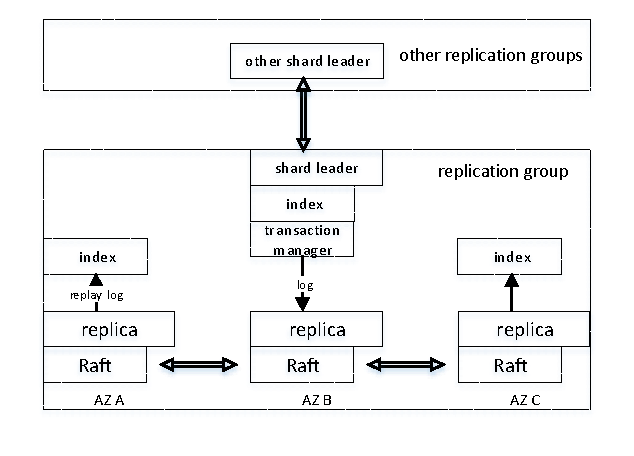
\includegraphics[scale=0.8]{figure/architecture.pdf}}
  \caption{Distributed and Replicated Database Architecture}
  \label{fig:architecture}
\end{figure}
The distributed commit and replication coordination protocol using chatty manner protocol enlarge the timespan of the critical path and amplified contention cost.
Figure~\ref{fig:architecture} presents the typical architecture.
First, the database partitions its data with many shards to scale.
Second, Each shard works on a replication layer which replicated data in several availability zones(AZ)\cite{Aurora:conf/sigmod/VerbitskiGSCGBM18} for high availability.
Between different available zones, the replication layer uses a consensus protocol to shield consistency.
\begin{figure}[htbp]
  \centerline{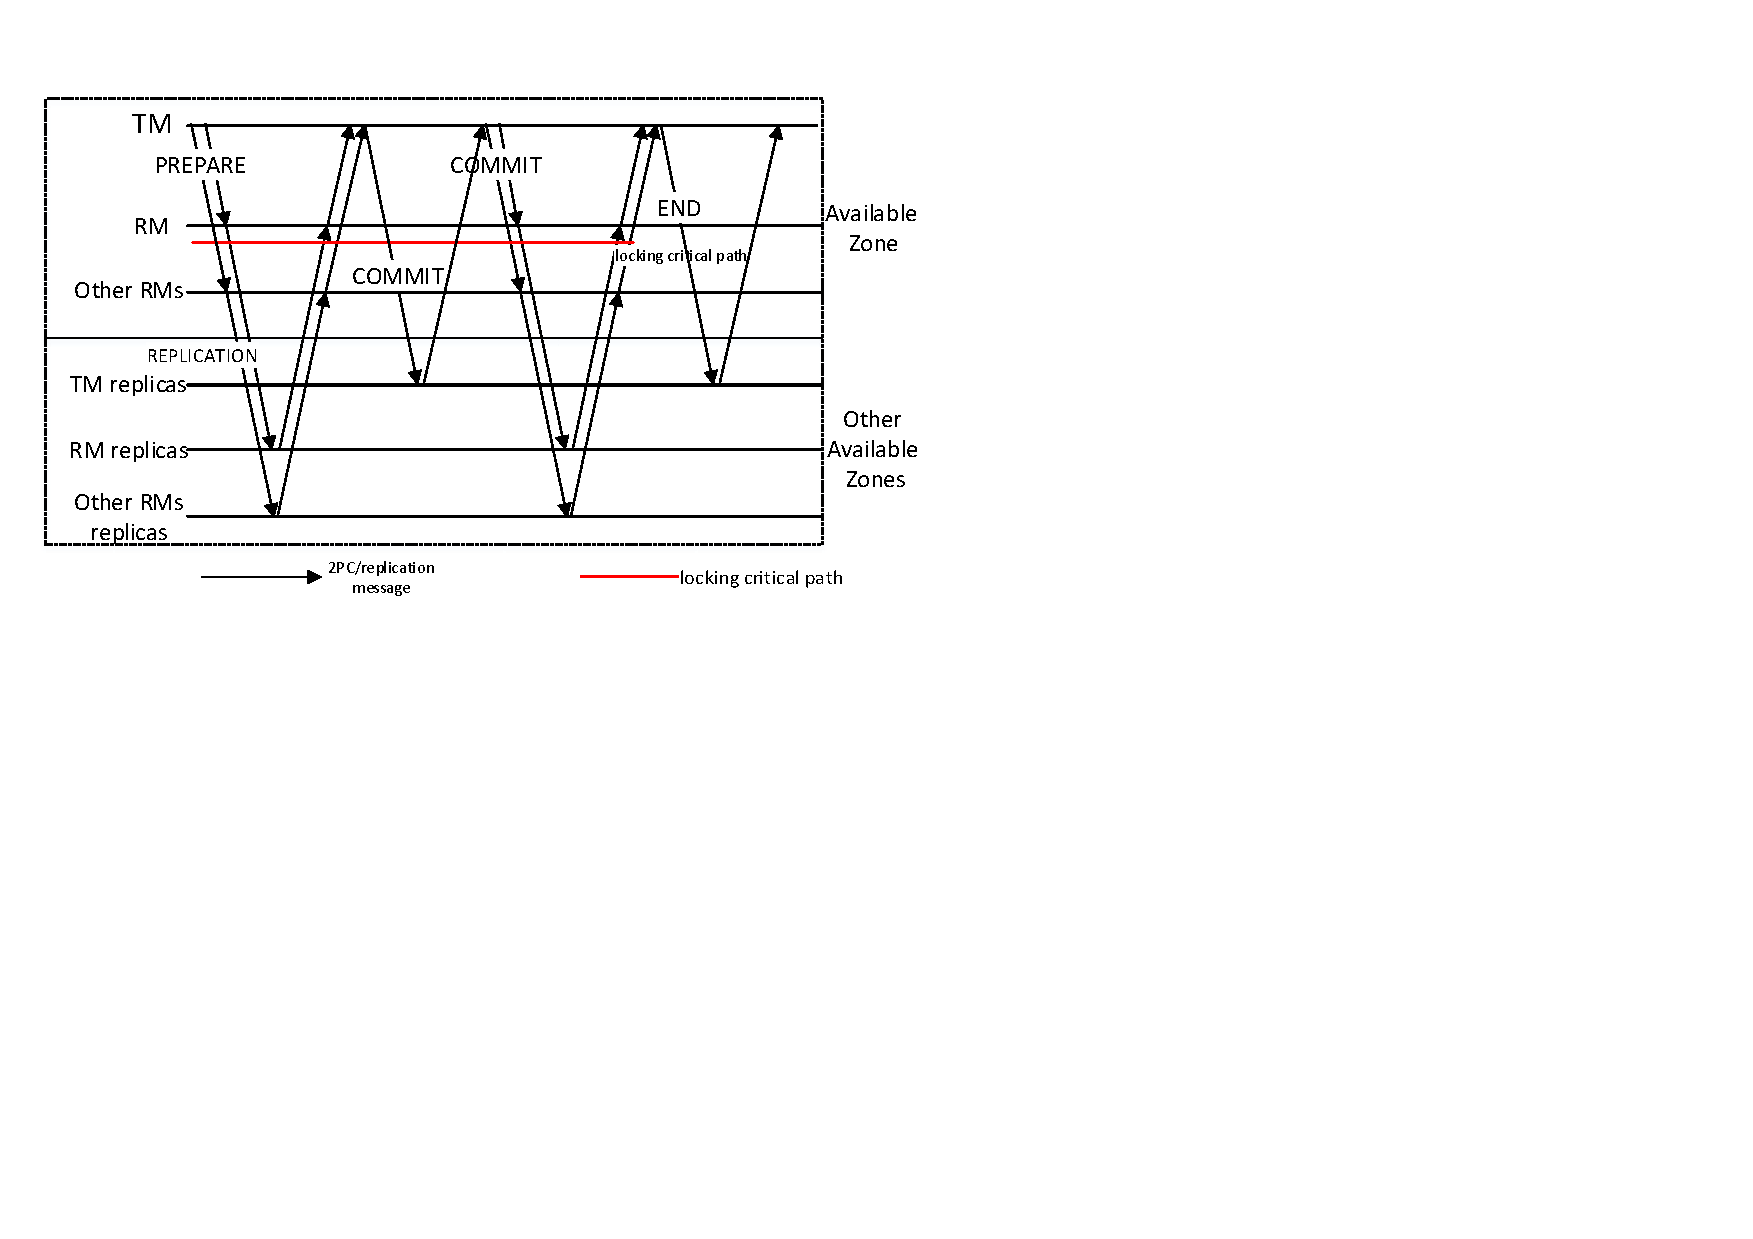
\includegraphics[scale=0.62]{figure/message_flow.pdf}}
  \caption{The message flow and lock hoding critical path of DB who uses 2PL(or with DLV ) and 2PC works on replication layer. 
The dash arrow line message is introduced by DLV. The red lines shows the critical path of S2PL and the green dash line shows the critical path of DLV.
  }
  \label{fig:two_layers_architecture}
\end{figure}

We focus on a on cloud distributed database using locking scheme and coordinater protocol on a replicated layer, especially who running transaction processing on geo-replicated layer.
Figure \ref{fig:two_layers_architecture} shows the message flow of a distributed transaction using S2PL and 2PC works on a WAN replication layer.
This architecture uses a chatty message protocol fails to scale high contention workload, as much previous work has discussed.
When a transaction requests its commit, \emph{TM(transaction manager)}  issues a prepare message to each \emph{RM(resource manager}).
\emph{RM} replicates its result to other replicas to make it fault tolerant.
\emph{RM} responses its decision to \emph{TM} after reach a consensus to guarantee fault tolerance. 
\emph{TM} then collects all the \emph{RMs} decisions.
And then it issues either a commit or abort decision to \emph{TM}'s replicas and
broadcast the final result to all \emph{RMs}.
Once a \emph{RM} receives the final result from \emph{TM}, it can release the locks that it had retained since it first accesses the specified tuple.
%We assume a distributed transaction \emph{T} access multiple \emph{RMs}, any other transaction \emph{T'} access any contended tuple \emph{x} locked would wait for \emph{T} to commit or abort.
%Transaction \emph{T} hold its lock from its first accessing a tuple to its finish(commit or abort).
%Transaction \emph{T'} would bocking its on the contented lock until \emph{t}finish.


We depict the lock duration with the red line in Figure~\ref{fig:two_layers_architecture} when commit.
The lock duration covers many message round trips including those over WAN.
Locking for generating a serializable order of concurrency operations is can be overly lengthy to commit contented transactions. 
Such a commit and replication protocol will severely impair the concurrency when confronted with a high degree of contention.
Previous works used speculative techniques, such as early lock release(ELR) \cite{EfficientLocking:conf/vldb/KimuraGK12}, controlled lock violation (CLV)\cite{CLV:conf/sigmod/GraefeLKTV13} to optimize transaction processing using locking.
These technique can be extended to distributed environment to increase concurrency.
Two layer architecture shares same bottleneck on force transaction log and faces even worse conditions.
Distributed transactions work on geo-replicated database need more time to write a log than non-distributed and non-replicated one.
However, extended these technique on distributed environment is complex.
There are some design considerations.
To combine two phase commit protocol, violate(or release) lock at which phase transaction.
As previous work addressed\cite{CLV:conf/sigmod/GraefeLKTV13}, violating lock at the first phase can exploit more concurrency but takes more dependency tracing cost and cascade abort cost.
Violating lock at the second phase may not exploit better concurrency but need maintain less dependency and get less cascade abort rate.
Transaction model, interactive or one-shot transactions may have different message flow, how different transaction types could benefit from these techniques?
Not all the transactions can benefit from CLV or ELR, little conflicts workloads are such cases.

In this paper, we propose a dynamic lock violation(DLV) to boost the locking-based distributed databases on cload, especially who are geo-replicated with a high commit latency.
DLV maintains less commit dependencies and bears less cascade abort penalty compares previous implementation\cite{CLV:conf/sigmod/GraefeLKTV13}. 
This section is the overall introduction of this paper.
Section \ref{sec:relate_work} is a review of related work.
Section \ref{sec:non_strict} presents a strict schedule is not necessary and hurt the performance of distributed and replicated databases.
Section \ref{sec:implement} introduces our speculative implementation.
Section \ref{sec:experiments} evaluates our experiment results.
Section \ref{sec:conclution} draws the conclusion of this paper.


\section{Relate Work}
\label{sec:relate_work}
This section introduces related work of this paper.

\subsection{Distributed Transaciton on Replicated Layer}
Recently, there are many scalable DBMS arised in both academia and industry.
Most of the systems in this category supports distributed query processing and
replicate data accross serveral data center geo-localted in diffferent areas for fault tolerance.
A fault-tolerant database relies on state-machine replication(SMR) log to avoid single point failure.
SMR needs to use a consensus protocol to enforce the same order of different replicas.
Paxos\cite{Paxos:journals/tocs/Lamport98}\cite{PaxosSimple:conf/opodis/Lamport02} is the most well-known consensus protocol.
Paxos use two messages round trip to accept a value, one roundtrip for choosing a proposal and another to propose the value.
Multidecree Paxos\cite{Multidecree:journals/csur/RenesseA15} elects a leader as the only proposer to eliminate Paxos first message roundtrip during normal processing.
Raft\cite{Raft:conf/usenix/OngaroO14} is a similar consensus protocol to Paxos, which is designed for understandability.
Consensus introduces significant overhead for its lots of message round trips and heavy network traffic.


Google spanner \cite{Spanner:conf/osdi/CorbettDEFFFGGHHHKKLLMMNQRRSSTWW12}\cite{Spanner:conf/sigmod/BaconBBCDFFGJKL17} is a geo-replicated and shared-nothing DBMS that uses hardware clock for timestamp generation.
VoltDB \cite{VoltDB} is a main memory database who runs single threaded execution per partition.
\cite{Calvin:conf/sigmod/ThomsonDWRSA12} use a deterministic transaction model, 
Calvin can commit distributed transaction without coordination protocol.
VolteDB and Calvin, by useing deterministic scheduling, they can use active replication to replicate transaction input rather than transaction effect.
Tapir\cite{Tapir:conf/sosp/ZhangSSKP15} and 


Although our work relies on Raft replication protocol, other replication protocols are also adequate since replication is an orthogonal system to database transaction processing.




\subsection{Locking Concurrency Control}
Database use concurrency control(CC) to calculate a concurrent schedule for concurrent transactions.
Two-phase locking(2PL) is the most widely used CC scheme.
As a pessimistic method, 2PL assumes that it is likely that transactions will conflict.
2PL uses a lock to enforce the order of conflicting transactions.
Strict 2PL(S2PL), in additional to 2PL, preserves its lock until a transaction's termination.
S2PL guarantees transaction's recoverability but a 2PL schedule cannot.
For enabling a simple recovery algorithm, most locking based databases choose S2PL.
When extending S2PL to distributed databases, S2PL can take more time blocking on its commit critical path for additional message round trips.

2PL protocol implementation varies on how to process deadlock.
In \emph{no-wait}
\cite{EvaluationOfCC:journals/pvldb/HardingAPS17}
policy, a transaction would imediantle abort the transction if it 
 fails to lock record. 
Previous work has prove it is the most scalabale technique to handle locking scheme, even in diestirbuted environment\cite{EvaluationCC1000Cores:journals/pvldb/YuBPDS14}\cite{EvaluationOfCC:journals/pvldb/HardingAPS17}.
Another policy is \emph{wait-die} \cite{LockNoWait:journals/csur/BernsteinG81} which is similar to \emph{no-wait}.
Transactions avoid to abort base on their start timestamps comparation when database using 2PL \emph{wait-die}.
In \emph{deadlock detection} \cite{LockCC:conf/ds/GrayLPT76},
transactions can wait for each other without controlling.
Transaction would abort only if there is a deadlock actually.
\emph{Deadlock detection} detect deadlock by explicitly tracing wait-for graph and testing circles.
Many traditional single node database\cite{MySQL}\cite{PostgreSQL} use \emph{deadlock detection} technique because it has no false positive abort. 
Deadlock detection on distributed database requires substential network messages to indentify circles and is  costly.


\subsection{Exploit Speculation and Lock Violation}
Exploit speculation is not a new idea.
Similar approaches have been introduced by many previous works.
Early lock release (ELR)
\cite{ELR:dewitt_implementation_1984}\cite{PS2PL:conf/icdt/Soisalon-SoininenY95}
\cite{Aether:journals/pvldb/JohnsonPSAA10}
\cite{EfficientLocking:conf/vldb/KimuraGK12}
\cite{Actor-Oriented-DB:conf/icde/Bernstein18}
shares the same idea with speculative approach. 
ELR can release transactions' lock without waiting for commit record flushed to disk.
DeWitt et al.\cite{ELR:dewitt_implementation_1984} firstly described ELR
 without implementation.
Soisalon-Soininen et al.\cite{PS2PL:conf/icdt/Soisalon-SoininenY95} proved that the correctness of ELR.
Johnson et al.\cite{Aether:journals/pvldb/JohnsonPSAA10} and\cite{EfficientLocking:conf/vldb/KimuraGK12} evaluated the performance improvement made by ELR.
Kimura et al.\cite{EfficientLocking:conf/vldb/KimuraGK12}\cite{Aether:journals/pvldb/JohnsonPSAA10} also address the weakness of previous ELR implementation\cite{ELR:dewitt_implementation_1984} can produce wrong results for read-only transactions.
Previous work exploits speculation mostly designed for single machine database system
\cite{PS2PL:conf/icdt/Soisalon-SoininenY95}
\cite{Aether:journals/pvldb/JohnsonPSAA10}
\cite{EfficientLocking:conf/vldb/KimuraGK12}.
Jones et al.\cite{LowOverheadCC:conf/sigmod/JonesAM10} use a restirct transaction model\cite{H-store:journals/pvldb/KallmanKNPRZJMSZHA08} implement sepculation.
Control lock violation(CLV)\cite{CLV:conf/sigmod/GraefeLKTV13} achieve the same performance as ELR but with a simple and general implementation.
CLV can apply to distributed databases and optimize both phases of two-phase commit.
CLV can use a ``register and report approach(RARA)''\cite{HeckatonMVCC:journals/pvldb/LarsonBDFPZ11} to implement its dependency.
RARA work well on a single-site database.
When RARA is used to process distributed transaction with no contention, the dependency tracing may be complex and costly.
More cascade abort rates on distributed transaction also lead more false positive violations and carry a performance penalty.

\subsection{Interactive Transaction and One-Shot Transaction}

Figure \ref{fig:transaction_type} shows the message flow of committing these two different type of transactions.
As shown in these figures, The interactive transaction needs more message roundtrips compared to one-shot one.
These two types of transaction model employ different speculative timing, which we will explain subsequently.

\begin{figure}[htbp]
    \centering
    \captionsetup[subfigure]{oneside,margin={0.3cm,0cm}}
    \subfloat[one-shot transaction, the red dotted lines show message added by \emph{DS}, when RM receive a \emph{Speculate} message, transaction can prevent deterministic abort. ]
        { 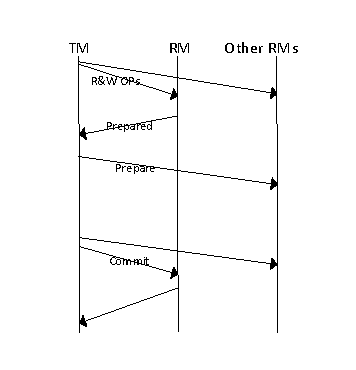
\includegraphics[scale=1] {figure/transaction_oneshot}  \label{fig:transaction_oneshot}  }
    \captionsetup[subfigure]{oneside,margin={0.3cm,0cm}}
    \subfloat[interactive transaction, when a RM receive a \emph{Prepare} message, transaction can prevent deterministic abort. ]
        { 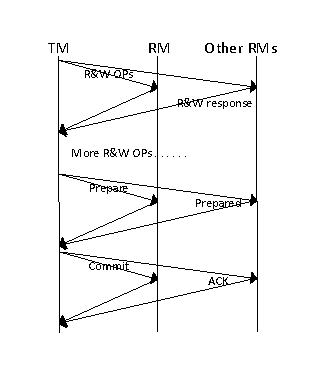
\includegraphics[scale=1]{figure/transaction_interactive} \label{fig:transaction_interactive}}
 
  \caption{One-shot distributed transaction and Interactive distributed transaction commit message flow}
  \label{fig:transaction_type} 
\end{figure}



\section{Beyond Strict Schedule And Lock Violation}.
\label{sec:non_strict}

In the following subsections, we descript our preliminaries and assumptions, the basic rule to keep transaction correctness when violating lock.

\subsection{Preliminaries And Assumptions}

The database shards its data by database primary keys.
Each shard replicated its physiological logs across different AZs for fault-tolerance.
The physiological logs record the row-level write operations of each transaction.
The replicated layer use Raft protocol to sustain consensus of log order. Other replication protocols may also work.
Only replica leader processes the transactional operations.
Both one-shot and interactive transactions are supported.

\subsection{Strict Scheduler Is Too "Strict" For Correctness But Too "Heavy" For Contention Workload}

Before we develop our method, we firstly review the formal definition of the transaction processiong operation.
Given a distributed transaction ${T_i}$,  it runs on ${m}$ sites  ${S = \{s_1, s_2, ... s_m\}}$.
The transaction history is a collection ${H = \{h_1, h_2, ..., h_m\}}$,
in which ${h_u (1 \le u \le m) = \Pi_u(H)}$ is the local history on site ${s_u}$.
${\Pi_u(H)}$ is ${H}$'s projection on site ${s_u}$.
For any projected history ${h_u(1 \le u \le m)}$, ${h_{u} }$ of transaction ${T_i}$ includes a collection of operations $o_i$.
$o_i$ can be read write operation, or command operations includes prepare commit(abort), abort or commit.
${r_i[x]}$ donates transaction ${T_i}$ reads record ${x}$,  ${w_i[x]}$ donates transaction ${T_i}$ writes record ${x}$.
${c_i}$, ${a_i}$, ${pc_i}$, ${pa_i}$ mean transaction ${T_i}$ commits, aborts, prepares commit or prepare abort respectively.
Transaction abort due to many reasons, they can be:
1.User request abort;
2.Violation of serializability;
3.Database node crash for failure.
We call the first two abort reasons \emph{deterministic abort} and the last \emph{non-deterministic abort}.

Transaction ${T_j}$ has a \emph{commit dependency} on transaciton ${T_i}$, written as ${T_j \rightarrow T_i}$, if ${T_j}$ can commit only if ${T_i}$ commit. 
If ${T_j}$ aborts, ${T_j}$ need also abort.
There are there kinds of dependencies, \emph{wr-dependency}, \emph{ww-dependency} and \emph{rw-dependency}.

If transaction ${T_i}$ and ${T_j}$ have direct write-read conflict on record ${x}$, in any local history ${h}$, ${T_j}$ read ${T_i}$'s write record,
we call this dependency read-write(wr) dependency and donated by ${w_i[x] \rightarrow r_j[x]}$.

Similarly, if ${T_i}$ and ${T_j}$ have direct write-write conflict on record ${x}$, ${T_j}$ overwrite ${T_i}$'s write record, this is  write-write(ww) dependency and written as ${w_i[x] \rightarrow w_j[x]}$.

And if ${T_i}$ and ${T_j}$ have direct read-write conflict on record ${x}$, ${T_j}$ write ${x}$ after ${T_i}$ reads ${x}$, it is a read-write(rw) dependency and recorded as ${r_i[x] \rightarrow w_j[x]}$. 
A transaction ${T_j}$ \emph{speculative access} a record ${x}$, if there is another transaction ${T_i}$, 
${T_j}$ has a commit dependency on ${T_i}$ and ${T_j}$ access ${x}$ before ${T_i}$ has committed.
We write this \emph{danger dependency} as ${w_j[x] \rightarrow_s r_i[x]}$, ${w_j[x] \rightarrow_s w_i[x]}$, 
${r_j[x] \rightarrow_s w_i[x]}$.
We also write ${T_j \rightarrow_s T_i}$ to indicate transaction ${T_i}$ has a commit \emph{danger dependency} on ${T_j}$. 


Traditional transaction schedulers choose strictness\cite{DBLP:conf/vldb/Raz92} to simplify implementation and avoid expensive transaction recovery cost.
Strictness implies that a transaction cannot read or overwrite a previous write by another transaction which has not ended yet.
For a locked base concurrency control scheme, the lock will hold until the transaction end, namely strict two-phase locking(S2PL).
Strictness is not necessary to produce a correct schedule.


Figure \ref{fig:strict_example} shows 3 transactions work 3 shards, ${S_1}$, ${S_2}$, ${S_3}$.
Ttheres are dependencies, ${r_1[x] \rightarrow w_3[x]}$, ${w_1[x] \rightarrow r_2[y]}$, ${r_2[y] \rightarrow w_3[x]}$ and there is ${T_1 \rightarrow T_2 \rightarrow T_3}$.
There is no circle in this dependency graph and the schedule is serializabile and strict. 
Figure~\ref{fig:non_strict_example} shows an example of a non-strict but correct schedule.
There is three records ${x}$, ${y}$, ${z}$, located at shard ${S_1}$, ${S_2}$, ${S_3}$.
Transaction ${T_1}$ execute write ${y}$, write ${x}$.
Transaction ${T_2}$ read ${T_1}$'s write on ${x}$ before ${T_1}$ commits.
Transaction ${T_3}$ overwrite ${T_2}$'s write ahead ${T_2}$'s commit.
The history ${H = \{h_1, h_2, h_3\}}$,
(in which, ${h_1=\{w_1[x]w_3[x]pc_1c_1pc_3c_3\}}$
${h_2=\{w_1[y]r_2[y]pc_1c_1pc_2c_2\}}$, 
${h_3=\{r_2[z]w_3[z]pc_2c_2pc_3c_3\} }$ )
is not a strict history, but it's a serializable history. 
Both of these two schedules are serializable equate with the serial schedule, ${T_1}$, ${T_2}$ and ${T_3}$.
Both scheule ${H_1}$ and ${H_2}$ are correct.


\begin{figure}[htbp]
  \centerline{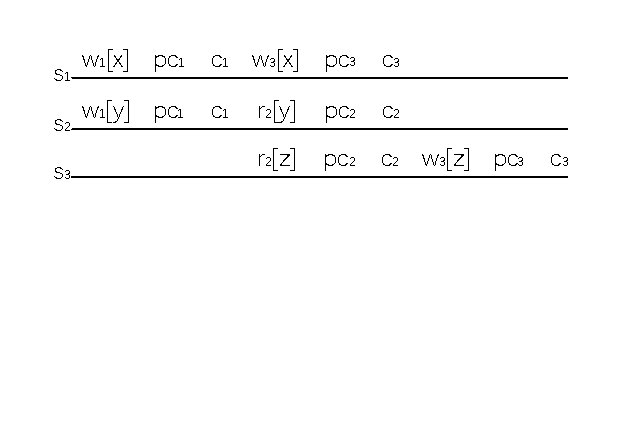
\includegraphics[scale=1]{figure/schedule_strict.pdf}}
  \caption{A strict and serializabile schedule ${H_1}$}
  \label{fig:strict_example}
\end{figure}

\begin{figure}[htbp]
  \centerline{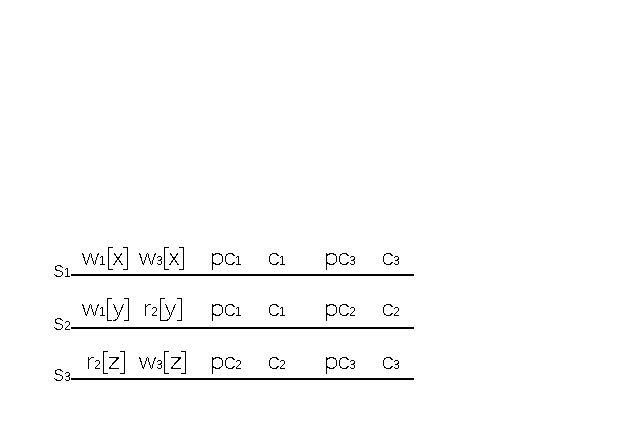
\includegraphics[scale=1]{figure/schedule_non_strict.pdf}}
  \caption{A non-strict but serializabile schedule ${H_2}$}
  \label{fig:non_strict_example}
\end{figure}

\begin{figure}[htbp]
  \centerline{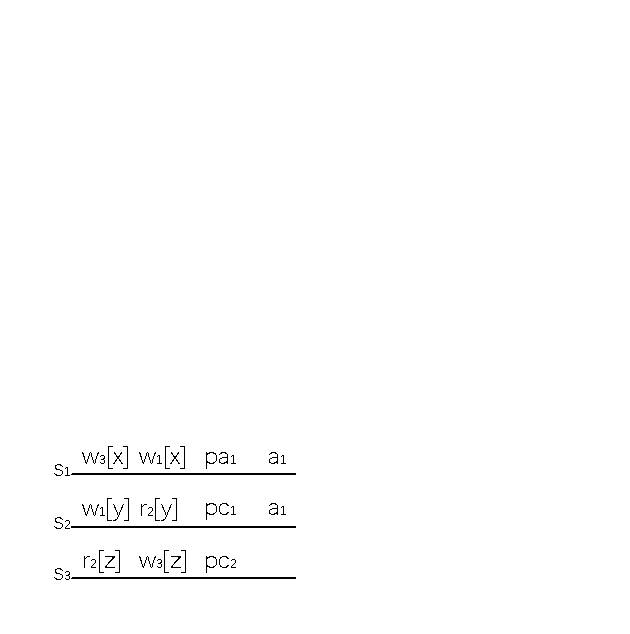
\includegraphics[scale=1]{figure/schedule_not_serializabile.pdf}}
  \caption{Schedule ${H_3}$, ${T_1}$ abort due to non-serializabile}
  \label{fig:schedule_abort_example}
\end{figure}

\begin{figure}[htbp]
  \centerline{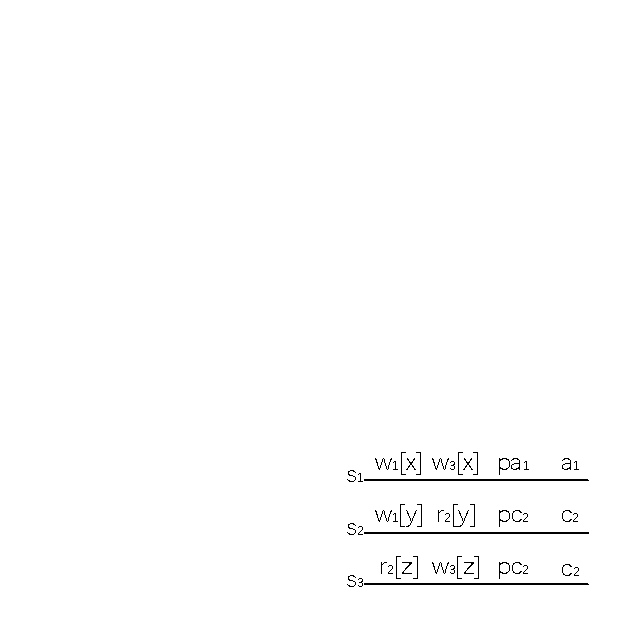
\includegraphics[scale=1]{figure/schedule_not_recoverable.pdf}}
  \caption{Schedule ${H_4}$, ${T_2}$ commit ahead ${T_1}$, non-recoverable anomaly}
  \label{fig:schedule_not_recoverable}
\end{figure}


To get better concurrency, the scheduler can produce schedule like ${H_2}$ in Figure~\ref{fig:non_strict_example}. 
Supporse schedule ${H_2}$ is created by locking, then transaction ${T_1}$ must release its locks or make its locks violatable before it knows its commit decision.
Then the following write or read cannot wait previous conflict access operations commit.
A transaction commits by no means an operation in a flash but progress that needs take lots of time.
Especially when it is a distributed commit on an RSM.
A distributed transaction need coordinating to decide an agreement on commit.
RSM need to reach consensus on every log record.
Strictness scheduler on a distributed and replicated database leads to a long critical path.
Our basic idea is to develop a serializable but non-strict correct scheduler for distributed transactions and shorten the critical path when commit.

A single node transaction can exploit log order to maintain dependency because dependent transactions write their logs orderly\cite{ELR:dewitt_implementation_1984}\cite{EfficientLocking:conf/vldb/KimuraGK12}.
When we extended non-strict locking protocol to a distributed transaction, transaction dependency maintaining is more complex.
If transactional scheduler can prevent all aborted transaction, the serializable scheduler is a correct one.
But when there is an aborted transaction, it does not.
To produce the correct log, the schedule must be both commit serializable and recoverable\cite{UnifyCR:journals/is/AlonsoVABASW94}.
Transaction need to maintains commit dependencies to guarantee serializabile and recoverable when exploit non-strictness.

\subsection{Lock Violating Rules and Dependency Tracing}

First, lock violation should produce a serializable schedule.
Take a schecule ${H_3}$ in Figure \ref{fig:schedule_abort_example} as an example.
There are danger dependencies.
${w_3[x] \rightarrow _s w_1[x]}$,
${w_1[y] \rightarrow _s r_2[y]}$,
${r_2[z] \rightarrow _s w_3[z]}$ in ${H_3}$.
There is a circle ${T_1 \rightarrow T_2 \rightarrow T_3 \rightarrow T_1}$.
This schedule is not serializable.
Transaction ${T_2}$
read from uncommitted transaction ${T_3}$.
When ${T_1}$ abort for non-serializable, ${T_2}$ must cascade abort to avoid anomaly.
If schedule ${H_3}$ is created by lock violation,
not formally, lock violation is just as a transaction releases its lock and another transaction acquire locks, then the locking is not two phases.
For a traditional locking scheme, transaction ${T_2}$ needs to wait for ${T_1}$'s release its lock until ${T_1}$ commit.
Transaction scheduler needs to trace commit dependencies and ensures dependency graph has no circles if a transaction violating locks of another conflict transaciton. 
%Before violating a transaction's lock, DLV prevent deterministic abort.
%DLV does not violate a transaction's lock only if the transaction can ensure it has no non-serializable error.
%A Transaction must avoid deterministic abort before it makes its lock violative.
%Avoid deterministic abort before lock violation is not only about correctness but also about performance.
%DLV has less dependency maintaining cost and cascade abort cost penalty by this way.
%DLV would not create a non-serializable schedule like ${H_3}$.

Second, lock violation must be recoverable.
In schedule ${H_4}$ of Figure~\ref{fig:schedule_not_recoverable}, 
${T_2}$ read from uncommitted transaction ${T_1}$'s write.
There is a danger dependency, ${w_1[y] \rightarrow_s r_2[y]}$ and ${T_2}$ 's commit is ahead ${T_1}$'s commit.
Schedule ${H_4}$ is non-recoverable.
If ${T_1}$ abort, then ${T_2}$ will return an error ${y}$ value.
The scheduler also need to maintain dependencies to keep schecule recoverable. 

There are serveral questions arised.
When should the transaction begin to violate lock?
How lock violation could composite with two phase protocol and different transaction models?
Violating lock at the first phase of two-phase can shorten more critical path and it isdesigned
is superior to
violating lock at the second phase.
But the database may bears more cascade aborts which are useless work.
DLV permits lock violation at two points in the timeline of running transactions.
We call these \emph{early-violation} and \emph{late-violation}.

\begin{center}
  ${H = l_i[x] o_i[x]... vl_j[x] o_j[x]...  l_i[y] o_i[y]... ul_i[x] ... }$
\footnote{

  $l_i[x]$:   ${T_i}$ lock tuple ${x}$
    
  $l_j[y]$:  ${T_j}$ lock tuple ${y}$
  
 $vl_j[x]$ : ${T_j}$ violating  ${T_i}$'s lock on ${x}$
 
 $ul_i[x]$: transaction ${T_i}$ release locks on ${x}$
}  
  , 
    
\end{center}




Suppose ${H}$ is a schedule which is created by lock violation, ${H}$ is extended by adding lock, unlock and lock violation operations.
If there is such $l_i[y]$ operations in schedule ${H}$,
then transaction ${T_j}$ is \emph{eraly lock violate} ${T_i}$'s lock on ${x}$;
otherwise, this is \emph{late lock violation}.
If a transaction use \emph{early lock violation}, it may lead to non-serializable schedule.
DLV needs maintains all $wr$, $ww$ and $rw$ dependencies after violating locks and guarantee the dependency graph of the schedule is acyclic. 
On the contrary, \emph{late lock violation} cannot make an acyclic dependency graph to become a cyclic one by adding any dependency edges.
This can be proved by formulating \emph{late lock violation} as 2PL proving.

Assume that there is a \emph{wr-dependency} from ${T_i}$ to ${T_j}$.
    ${T_j}$, which can be written as ${w_i[x] \rightarrow r_j[x]}$.
${T_j}$ cannot commit if ${T_i}$ has not committed.
Traditional S2PL schedule can guarantee this by release locking when ${T_i}$ commit.
Lock violating violates locking rule and ${T_j}$ can read ${T_i}$'s write on ${x}$ before ${T_i}$ commits.
In lock violation case, transactions must tracing dependencies and commit as dependency orders. 
Composite with 2PC protocol, we have the following rules:

\begin{enumerate}
  \item ${T_i}$ prepares only if ${T_j}$ commit;
  \label{rule:prepare}

  \item  ${T_i}$ commits only if ${T_j}$ commit;
  \label{rule:commit} 
  
  \item If ${T_j}$ aborts, ${T_i}$ must also abort

  \label{rule:abort} 
    \end{enumerate}

By tracing dependencies after violating a lock, DLV schedule achieves both serializabile and recoverable.

\section{DLV implementation}.

\subsection {In Memory Speculative Versions}

Non-strict scheduler needs more complex recovery algorithm to keep correctness.
Take a schedule ${H}$ as an exapmple,


\begin{center}
${H = w_1[x]w_1[y]r_2[x]w_2[y]a_1a_2}$

\end{center}

If transaction ${T_1}$ abort, this cause cascade abort.
Traditional database use undo log to process recovery transaction write operations.
Implementation undo maybe a little tricky when using exploint non-strict.
A wrong recovery expand schedule of ${T_1}$ may be like ${exp(H)}$,
in which ${w^-_i[x]}$ means transaction ${T_i}$ undo its write on ${x}$.
\begin{center}
  
  ${exp(H) =  w_1[x]w_1[y]r_2[x]w_2[y]}$
  ${w^-_1[y]w^-_1[x]c_1w^-_2[y]c_2}$
\end{center}
Suppose the initial value of ${x}$ and ${v}$ of are both ${0}$. The value of ${x}$, ${y}$ after executing every operations in $exp(H)$ is shown in Table~\ref{tbl:x_y_vlues}.
The final value of ${y}$ is 1, which should be 0.


\begin{table}[htb]
  \centering
  \begin{tabular}{|c|c|c|c|c|c|}
  \hline
operations & x &  y & undo   \\ 
  \hline
  \hline
  $w_1[x=1]$ & 1 & 0 & x=0  \\ 
  \hline
  $w_1[y=1]$ & 1 & 1 & y=0   \\
  \hline
  $r_2[x]$ & 1 & 1 &    \\
  \hline
  $w_2[y=2]$ & 1 & 2 & y=1  \\
  \hline
  $w^-_1[y=0]$ & 1 & 0 &   \\
  \hline
  $w^-_1[x=0]$ & 0 & 0 &   \\
  \hline

  $c_1$ & 0 & 0 &   \\
  \hline
  $w^-_2[y=1]$ & 0 & 1 &    \\
  \hline
  $c_2$ & 0 & 1 &  \\
  \hline
  \end{tabular}
\caption{x, y values, undo log after the execution of ${exp(H)}$}
\label{tbl:x_y_vlues}
\end{table}

To tackle this anomaly, recovery must make more complex algorithm such as SOT\cite{UnifyCR:journals/is/AlonsoVABASW94}.
For schedule ${H}$, a correct recovery expandation may be: 
\begin{center}
${exp^*(H) = w_1[x]w_1[y]r_2[x]w_2[y]w^-_2[y]c_2w^-_1[y]w^-_1[x]c_1}$
\end{center}
The schdeuler must recovery transaction by the reserve order of write operation.
If ${x}$ and ${y}$ is on the same database node and transaction is a single node one, to generate this expanding schedule, recovery algorithm can simply execute undo operation follow as log's reserve order, just like traditional Aries algorithm does.
However, if ${x}$ and ${y}$ are not located at the same node, this undo operation order is hard to accomplish because of partial failure.

In order to avoid this complexity , DLV maintains uncommitted speculative versions in memory and obeys no-steal policy when writting data.
No-steal policy need storage cannot write  uncommitted data to permernant storages.
Since no-steal policy is designed for space efficiency.
For most transactions would write a little data excpet the bulk loading ones and
modern database runs on a machine with large RAM, using no-steal policy is not necessary. 
By no-steal and speculative versions, the database needs no undo log, transaction rollback and failure recovery would be more simple and efficiency.
DLV 's speculative version implementation is a little similar with many multi-version concurrency control scheme.
The list is structured from the newest version to the oldest version and the last version of this list is the committed version.
Speculation versions are always stored in main memory and needs no persistence.
If a transaction would abort, it only needs to remove its write versions from speculative version list.

Previously , we have discussed that a \emph{ww} dependency has no effect on recoverability.
\emph{Late-violation}, since it has promised serializability, so it can ignore ${ww}$ and ${rw}$ dependencies and only trace ${wr}$ dependencies for recoverability.
Figure~\ref{fig:versions_example} show a series of schedule access on two contention rows, ${x}$, ${y}$.
The green rectangles are speculative versions and the red ones are committed versions.
Although there is ${ww}$ dependency ${w_6[x] \rightarrow w_4[x]}$.
The abort of $T_4$ does not cause ${T_6}$ cascade abort.
\begin{figure}[htbp]
  \centering
  \captionsetup[subfigure]{margin={0cm,0cm}}
  \subfloat[\small ${H_a = w_1[x_0]w_1[y_0]c_1w_2[x_1]w_3[x_2]w_3[y_1]w_4[x_3]}$]
  { 
    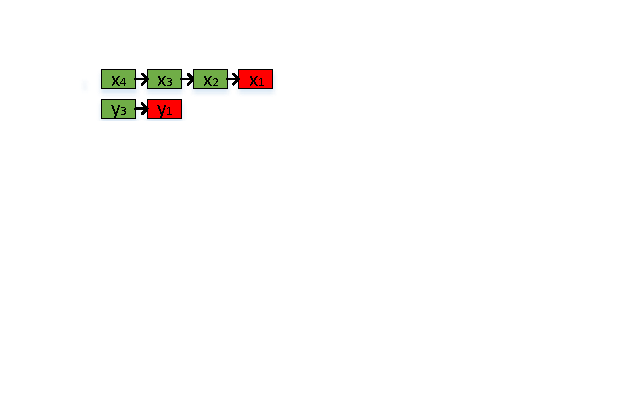
\includegraphics[scale=1.5] {figure/version1} \label{fig:versions_a}}
    \captionsetup[subfigure]{margin={0cm,0cm}
  }
  \subfloat[\small ${H_b = H_a c_2r_5[y_3]r_6[x_4]}$]
  { 
    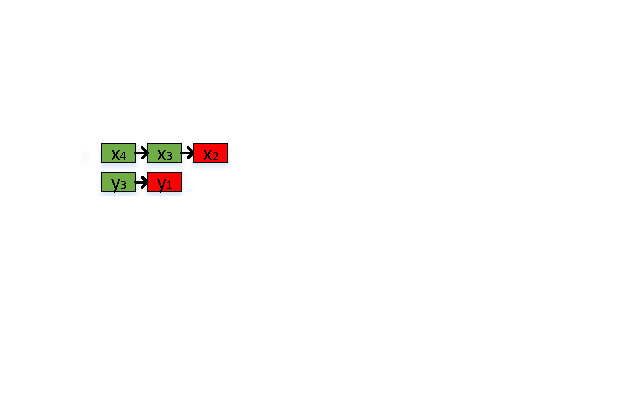
\includegraphics[scale=1.5]{figure/version2} \label{fig:versions_b}
  }
    \captionsetup[subfigure]{margin={0cm,0cm}
  }
  \subfloat[\small ${H_c = H_b a_3a_5}$]
  { 
    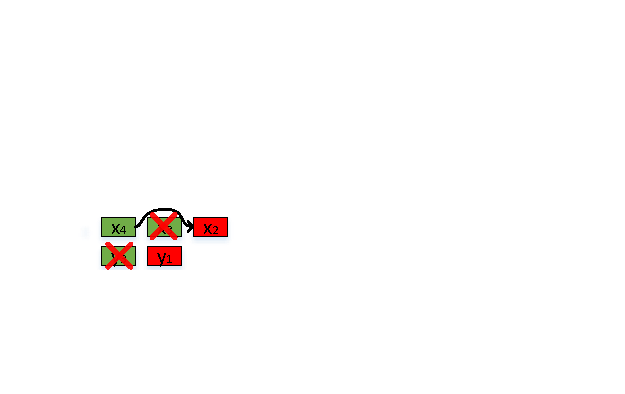
\includegraphics[scale=1.5] {figure/version3} \label{fig:versions_c}}
    \captionsetup[subfigure]{margin={0cm,0cm}}
    \subfloat[\small ${H_d = H_c c_4r_6[y_1]c_6}$]
      { 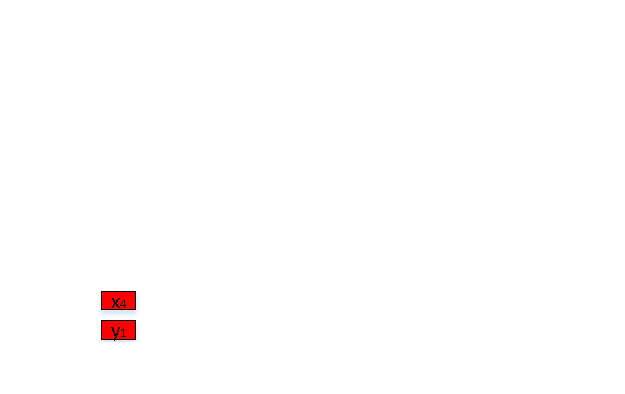
\includegraphics[scale=1.5]{figure/version4} \label{fig:versions_d}
  }
  \caption{speculative(green) and committed(red) versions, 
  ${x_i}$ , ${y_i}$ express this version is from transaction transaction ${T_i}$'s write
}
\label{fig:versions_example}
\end{figure}

\iffalse
To specify a contention, every transaction context keeps a wait counter.
If ${T_j}$ waits a lock on a row which is write locked by ${T_i}$, ${T_j}$ will add this wait counter by one. 
This wait counter record how many blocking transactions are waiting for this transaction's write lock.
Once the wait counter exceeds a limitation, support this value is ${\Theta}$, we identify this transaction is contented transactions.
Only if a transaction is a contented transaction,  it can exploit speculation.
\fi

\subsection {Dynamic Decide Early or Late Violation}
\emph{Early-violation} can is more appropriate then \emph{Late-violation} when there are less cascade abort caused by non-deterministic abort.
\emph{Early-violation} also need more dependency tracing costs.
Too many cascade abort can lead a lot useless work.

We implementation \emph{Late-Violation} by adding a message round trip to prevent deterministic abort.
This additional message flow shows in Algorithm~\ref{alg:speculate_phase}.
In Figure~\ref{fig:two_layers_architecture}, the message is show as dotted arrow lines.
Before an ${RM}$ decides to replicate its prepare log, it also send a \emph{Ready} message to ${TM}$ and tells ${TM}$ its will prepare this transaction.
\emph{Ready} message shows that the ${RM}$ will prepare commit or prepare abort.
When the \emph{TM} collect all \emph{RM}s \emph{Ready} message, it sends \emph{Violate} messages to tells every \emph{RMs} make their locks violatable.
An interactive-transaction can combine these messages with the last operations and prepare requests in passing, as Figure~\ref{fig:transaction_type} shows.
For a oneshot transaction, this message flow also takes less time than the overall message flow of 2PC because of no log replication time dealy.
Especially when all the ${RMs}$ and the ${TM}$ are located in LAN, there is no WAN message needed. 

DLV records transaction statistic information to decide use \emph{early-violateion} or \emph{late-violation}.
We define a distributed transaction working on one ${RM}$ as partial transaction and a partial transaction enter prepared commit phase but failed to commit finally as partial prepare.
DLV calculates partial prepare rate at a time period to decide which violation strategy to choose.
We supporse that a transaction ${T}$ running at time ${\tau}$ would access a collection of shards
${S_1, S_2, ..., S_n}$. 
The message-round trip time from ${T}$'s ${TM}$ to ${RM}$ on shard ${S_i}$ is ${RTT_i}$.
In a window period time from ${\tau - \delta}$ to ${\tau}$, there is ${N_p}$ partial preapres of total ${N_t}$ partial transactions. 
DLV would tests following conditions where ${\Theta}$ is is a constant coefficient. 

\begin{center}
  ${N_p / N_t < \Theta * max(RTT_i)}$
\end{center}

DLV would choose \emph{early-violation} if this conditions stisfied. 
Otherwise it would use \emph{late-violation}.


\subsection {Locking Violation and Maintain Commit Dependency}
DLV use \emph{wait-die} protocol to avoid deadlock.
At the beginning of a transaction, the transaction current timestamps to generate a transaction id.
The conflict transaction operation are queued base their transaction id's order. 


\emph{DS} use register and report\cite{HeckatonMVCC:journals/pvldb/LarsonBDFPZ11} to maintain dependency.
Every transaction content store an in dependency transaction(${in\_dn}$) number record how many transactions is the transaction dependent on.
The transaction also keeps an out transaction set(${out_set}$) attribute record the transactions depend on it.
When a transaction ${T}$ speculative read from ${S}$.
${T}$ registers dependency from ${S}$ by adding ${T}$ to ${out\_set}$ of ${S}$ and increase ${in\_dn}$ of ${T}$ by one.
This steps are described by line 4 ~ 7 in function READ \ref{func:read}.
A transaction cannot prepare if it's ${in\_dn}$ value is greater than 0, which means some in dependency transaction does not commit yet.
If a transaction's ${in\_dn}$ value is less than 0, the transaction must abort because there is some in dependency abort cause a cascade abort.
Algorithm~\ref{alg:prepare_phase} shows how to prepare a transaction.
When a transaction commits, this transaction would traversal its ${out\_set}$ and decrease every transaction's ${in\_dn}$ by one, this is shown in line 6~10 of COMMIT \ref{func:commit} function.
If a transaction aborts, it may cause a cascade abort.
Line 2 of function CASCADE \ref{func:cascade} shows the assign ${in\_dn}$ by a negative value when cascade abort.

\subsection{Pseudocode Description}

Algorithm~\ref{alg:execution_phase} shows the execution phase of a transaction. 
Algorithm~\ref{alg:prepare_phase} shows the prepare phase of a transaction. 
Algorithm~\ref{alg:commit_phase} shows the commit phase of a transaction. 
Algorithm~\ref{alg:speculate_phase} shows the speculation phase of a transaction. 
\begin{algorithm}[!h]

  \caption{Execution phase of transaction ${T}$. Read and write a key}
  
  \begin{algorithmic}[1]
  \Function{Read}{$T,key$}
      \State ${newest\_version \gets Head(Tuple(key).version\_list)}$
      \If {${newest\_version}$ is created by transaction ${S}$ \newline \textbf{and} ${key}$ is ICommit locked by ${S}$ }
        \If {${T \notin S.out\_set }$}
          \State ${S.out\_set \gets S.out\_set \cup T}$
          \State ${T.in\_dn \gets T.in\_dn + 1}$
        \EndIf 
      \EndIf
      \If {${key}$ is \emph{write} locked by transaction ${S}$}
        \State ${S.wait \gets S.wait + 1}$
        \State wait lock till die
        \If {die}
            \State ${T.no\_da \gets }$ \textbf{False}
            \State \textbf{return} die error.
        \EndIf
      \EndIf
      \If {${key}$ is \emph{IAbort} locked by transaction ${S}$}
        \State wait lock this lock released
      \EndIf
      \State Lock(${T, key, Read}$)
      \State \textbf{return} ${key}$'s value.
      \label{func:read}
  \EndFunction
  \end{algorithmic}


  \begin{algorithmic}[1]
  \Function{Write}{$T,key, value$}
    \If {${key}$ is \emph{read} or \emph{write} locked}
      \If {${key}$ is \emph{write} locked by transaction ${S}$}
        \State ${S.wait \gets S.wait + 1}$
      \EndIf
      \State wait lock till die
      \If {die}
        \State ${T.no\_da \gets }$ \textbf{False}
        \State \textbf{return} die error.
      \EndIf
    \EndIf
    \State Lock(${T, key, Write}$)
    \State add a new version of ${key}$'s tuple, assign ${value}$
  \label{func:write}
  \EndFunction
  \end{algorithmic}
  \label{alg:execution_phase}
\end{algorithm}

\begin{algorithm}[!h]
  \caption{Prepare phase of transaction ${T}$}
  \begin{algorithmic}[1]
  \Function{Prepare}{$T$}
    \State wait if ${T.in\_dn > 0}$
    \If {${T.in\_dn < 0}$}
      \State response \emph{TM} message \emph{\{Prepare Abort\}}
    \ElsIf {$T.in\_dn = 0$}
      \State response \emph{TM} message \emph{\{Prepare Commit\}} \newline or \emph{\{Prepare Abort\}}
    \EndIf 
  \EndFunction
  \end{algorithmic}
  \label{alg:prepare_phase}
\end{algorithm}

\begin{algorithm}[!h]
  \caption{Commit phase of transaction ${T}$, commit and (cascade)abort function}
  \begin{algorithmic}[1]
  \Function{Commit}{$T$}
    \State garbage collect old version in \newline ${Tuple(key).version\_list}$
    \For {$ key \in T.write\_set \cup T.read\_set$}
      \State Unlock(${T, key, Read/Write}$)
    \EndFor
    \For {${T_{out} \in T.out\_set}$} 
      \State ${T_{out}.in\_dn \gets T_{out}.in\_dn - 1}$ \Comment{keep exactly once}
      \If ${T_{out}.in\_dn = 0}$ 
        \State report ${T_{out}.in\_dn = 0}$ \Comment{ stop waiting on function PREPARE line 2}
      \EndIf
    \EndFor
    \State response \emph{TM} message \emph{\{Commit ACK\}}
    \label{func:commit}
  \EndFunction
  \end{algorithmic}
  \begin{algorithmic}[1]
  \Function{ABORT}{$T$}
    \State \textbf{call} CASCADE(T)
    \For {$ key \in T.write\_set \cup T.read\_set$}
      \State Unlock(${T, key, Read/Write}$)
    \EndFor
    \State response \emph{TM} message \emph{\{Abort ACK\}}
    \label{func:abort}
  \EndFunction
  \end{algorithmic}
  \begin{algorithmic}[1]
    \Function{CASCADE}{$T$}
      \State ${T.in\_dn \gets -\infty }$
      \For {$ key \in T.write\_set$}
        \If {$key$ is ${ICommit}$ locked by ${T}$}
          \State ModifyLock($T, key, IAbort$)
        \EndIf
        \For {${version \in Tuple(key).version\_list}$}
          \If {${version}$ is created by ${T}$}
            \State remove ${version}$ from list
            \State \textbf{break}
          \EndIf 
        \EndFor
      \EndFor
      \For {${T_{out} \in T.out\_set}$} 
        \State \textbf{call} CASCADE(${T_{out}}$)
      \EndFor
      \label{func:cascade}
    \EndFunction
  \end{algorithmic}
  \label{alg:commit_phase}
\end{algorithm}

\begin{algorithm}[!h]

  \caption{Speculate phase. \
  \newline
  \emph{Ready} and \emph{Speculate} works on \emph{RM}.
  \newline
  \emph{TM} call \emph{Decide} send when \emph{TM} collects all \emph{RM}'s \emph{Ready} message.
  \newline
  \emph{msgs} is a collection of \emph{Ready} message which TM receives from all the \emph{RM}s.
  \newline
  ${\Theta}$ is a threshhold value to enable speculation.}
  \begin{algorithmic}[1]
  \Function{Ready}{$T$}
      \State response \emph{TM} message \newline \emph{\{Ready, ${wait \gets T.wait}$, ${non\_da \gets T.non\_da}$\}}
  \label{func:ready}
  \EndFunction
  \end{algorithmic}
  \begin{algorithmic}[1]
  \Function{Decide}{$T, msgs$}
    \If{${\forall m \in msgs}$, ${m.non\_da}$ is \textbf{True} \textbf{and} \newline
    ${\exists m \in msgs}$, ${m.wait > \Theta}$ }
      \State send all \emph{RM}s message \emph{\{Speculate\}} 
    \EndIf
  \label{func:decide}
  \EndFunction
  \end{algorithmic}
  \begin{algorithmic}[1]
  \Function{Speculate}{$T$}
    \For {$ key \in T.read\_set$}
      \State Unlock($T, key, Read$)
    \EndFor
    \For {$ key \in T.write\_set$}
      \If {$key$ is ${Write}$ locked by ${T}$}
        \State ModifyLock($T, key, ICommit$)
      \EndIf
    \EndFor
  \label{func:speculate}
  \EndFunction
  \end{algorithmic}
  \label{alg:speculate_phase}
\end{algorithm}

\section{Experiments and Evaluations}
\label{sec:experiments}
We develop a replicated distributed database demo and evaluate the performance of \emph{DS}.
As a comparison with \emph{DS}, we also implement S2PL wait die(S2PL) scheme, CLV optimize both violate at the 1st phase(CLV1P) and 2nd phase(CLV2P).

\subsection{Experiments Setting}
Our experiments performed on a cluster of 12 Aliyun ecs.g6.large server.
Each server has 2 virtual CPU with 2.5GHz clock speed, 8GB RAM, runs Ubuntu 16.04.
The data is partitioned by 4 shards, each shard has 3 replicas which is replicated across 3 AZs.
Every AZ has a full data copy of each shard.
The internal network bandwidth of each AZ is 1Gbps.
We choose a modifies version TPCC workload who has 60\% NewOrder procedure and 40\% Payment procedure.
All the transactions are distributed transactions.
The data set has 20 warehouse number and shard by warehouse id.
Each transaction will retry after 3 seconds if it aborts.

\subsection{Performance Comparation}
Figure \ref{fig:add_terminal_gathered_mode} shows the performance of when adding terminal numbers of each node in the gathered mode
(TMs and RMs are located in the same AZ).
In Figure \ref{fig:tps_add_terminal}, we can see \emph{DS} scales better than the other algorithms.
CLV2P has little optimization against S2PL.
CLV1P has grater abort rates,  as \ref{fig:abort_add_terminal} shows, and has bad performance.
Figure \ref{fig:add_terminal_scathered_mode} shows the performance of when adding terminal numbers of each node in scattered mode.
(TMs and RMs are located in the different AZs).


\begin{figure*}[htbp]
  \centering
  \captionsetup[subfigure]{margin={0cm,0cm}}
  \subfloat[one-shot transaction TPS of different terminal numbers]
      { 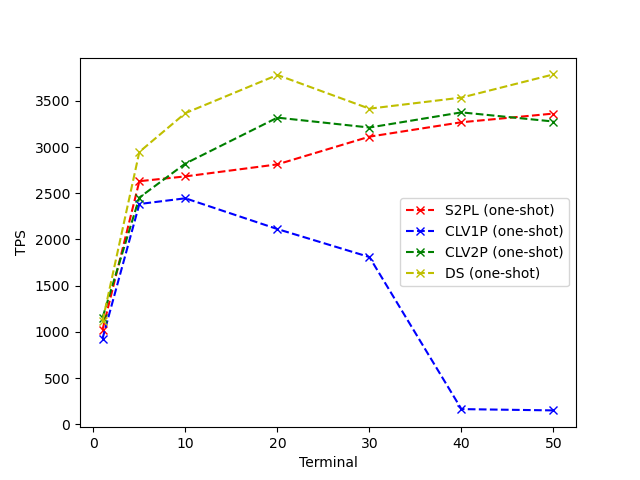
\includegraphics[scale=0.25] {figure/tps_plot_add_terminal} \label{fig:tps_add_terminal}}
  \captionsetup[subfigure]{margin={0cm,0cm}}
  \subfloat[one-shot trnasaction abort rate of different terminal numbers]
      { 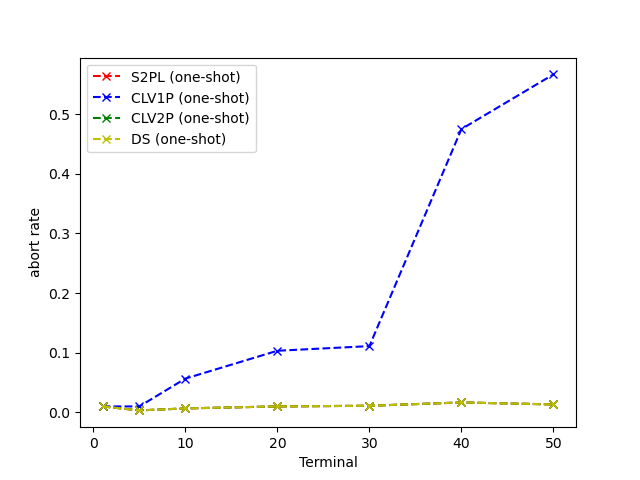
\includegraphics[scale=0.25]{figure/abort_plot_add_terminal} \label{fig:abort_add_terminal}}
  \captionsetup[subfigure]{margin={0cm,0cm}}
  \subfloat[interactive transaction TPS of different terminal numbers (TODO) ]
      { 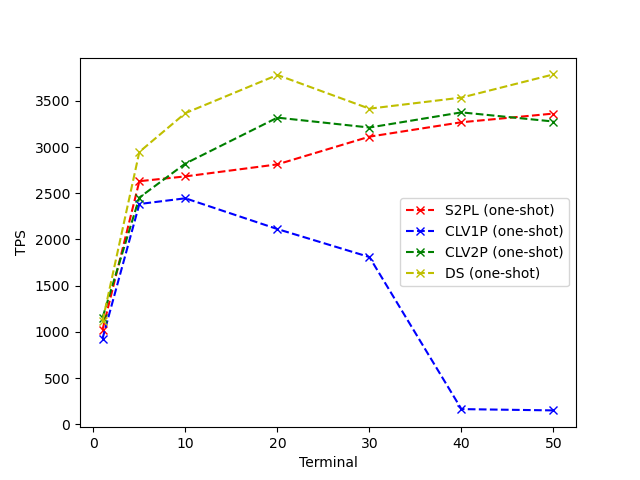
\includegraphics[scale=0.25] {figure/tps_plot_add_terminal} \label{fig:tps_add_terminal}}
  \captionsetup[subfigure]{margin={0cm,0cm}}
  \subfloat[interactive trnasaction abort rate of different terminal numbers (TODO)]
      { 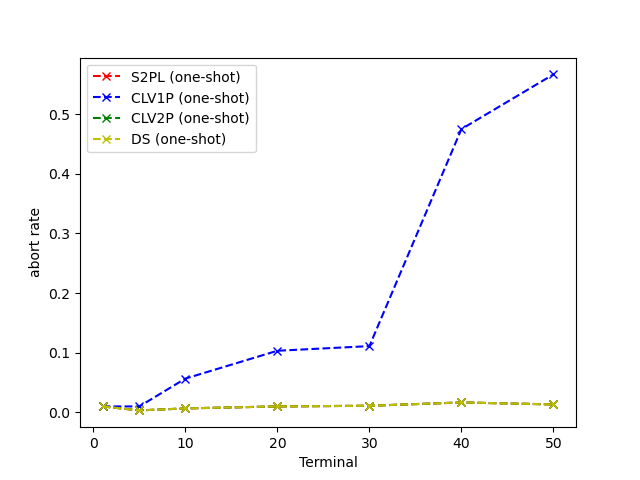
\includegraphics[scale=0.25]{figure/abort_plot_add_terminal} \label{fig:abort_add_terminal}}
\caption{throughput and abort rate when adding terminal number of each node, gathered mode}
\label{fig:add_terminal_gathered_mode}
\end{figure*}

\begin{figure*}[htbp]
  \centering
  \captionsetup[subfigure]{margin={0cm,0cm}}
  \subfloat[one-shot transaction TPS of different terminal numbers (TODO)]
      { 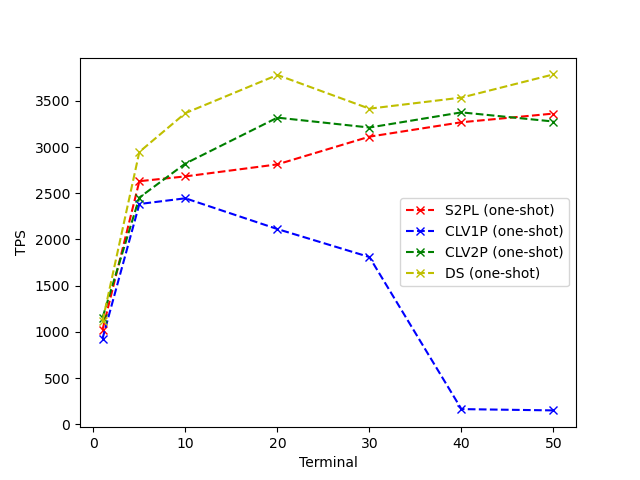
\includegraphics[scale=0.25] {figure/tps_plot_add_terminal} \label{fig:tps_add_terminal}}
  \captionsetup[subfigure]{margin={0cm,0cm}}
  \subfloat[one-shot trnasaction abort rate of different terminal numbers (TODO)]
      { 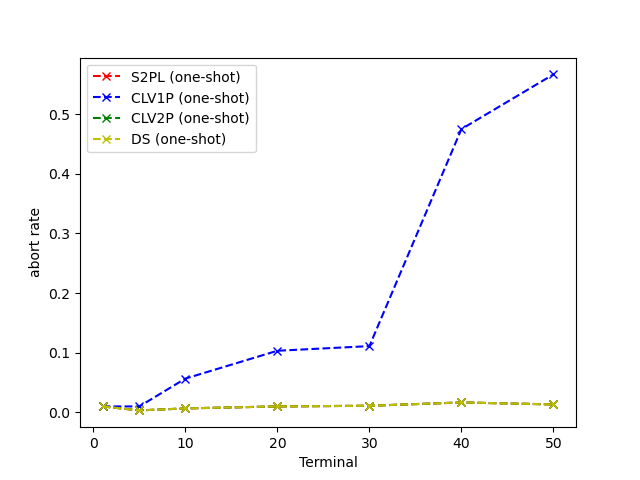
\includegraphics[scale=0.25]{figure/abort_plot_add_terminal} \label{fig:abort_add_terminal}}
  \captionsetup[subfigure]{margin={0cm,0cm}}
  \subfloat[interactive transaction TPS of different terminal numbers (TODO) ]
      { 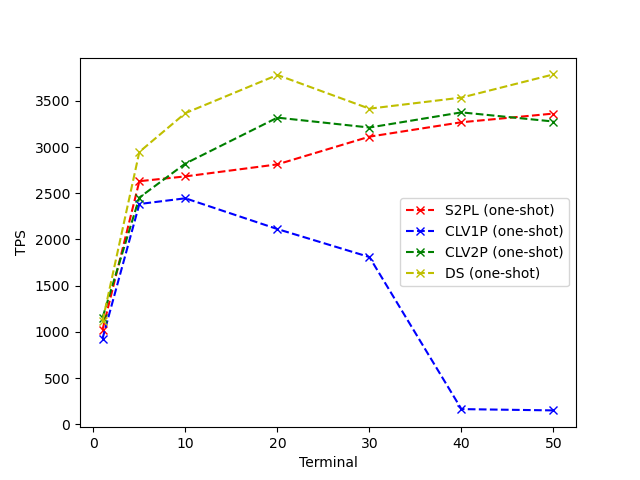
\includegraphics[scale=0.25] {figure/tps_plot_add_terminal} \label{fig:tps_add_terminal}}
  \captionsetup[subfigure]{margin={0cm,0cm}}
  \subfloat[interactive trnasaction abort rate of different terminal numbers (TODO)]
      { 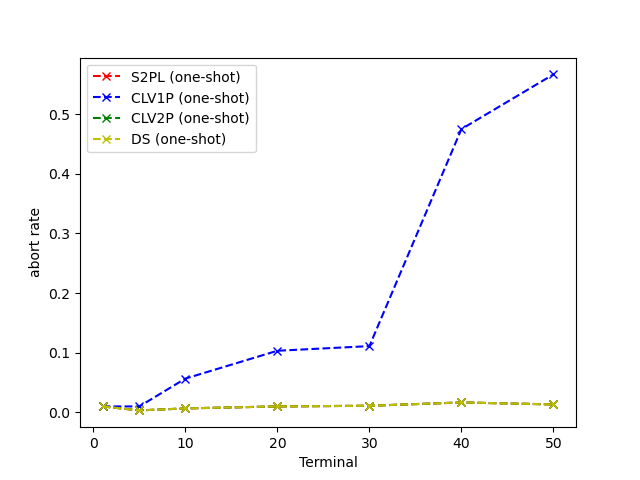
\includegraphics[scale=0.25]{figure/abort_plot_add_terminal} \label{fig:abort_add_terminal}}
\caption{throughput and abort rate when adding terminal number of each node, scathered mode}
\label{fig:add_terminal_scathered_mode}
\end{figure*}


\begin{figure}[htbp]
  \centering
  \captionsetup[subfigure]{margin={0cm,0cm}}
  \subfloat[transaction TPS of different contention rate (TODO)]
      { 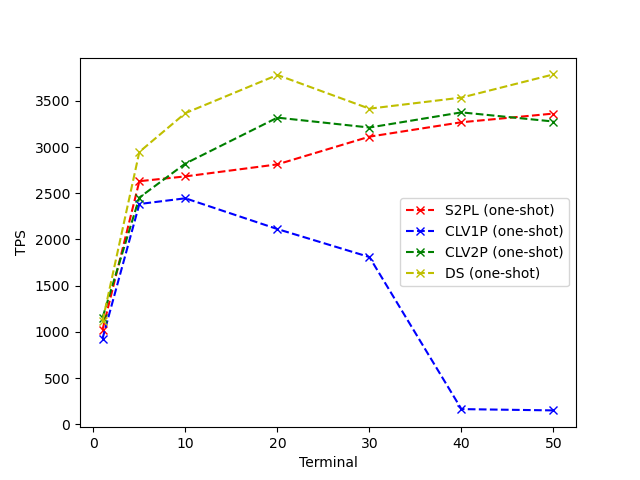
\includegraphics[scale=0.24] {figure/tps_plot_add_terminal} \label{fig:tps_add_terminal}}
  \captionsetup[subfigure]{margin={0cm,0cm}}
  \subfloat[trnasaction abort rate of different contention rate (TODO)]
      { 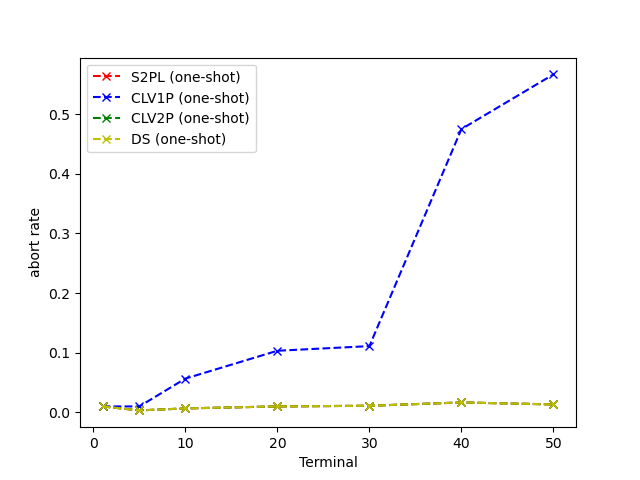
\includegraphics[scale=0.24]{figure/abort_plot_add_terminal} \label{fig:abort_add_terminal}}
\caption{throughput and abort rate when adding possible contention}
\label{fig:add_terminal_scathered_mode}
\end{figure}



\subsection{Parameter Tune}

\subsection{Recovery Non-Available Time Comparation}

\section{Conclution}
\label{sec:conclution}
We develop $DS$ optimization for locking scheme on cloud distributed database.
${DS}$'s speculation is only available if it is worthy.
According to our evaluation, ${DS}$ can improve performance of contention workload for shortening critical path.
It also avoids unnecessary dependency tracing cost and cascade abort danger when encounter non-contention workload compares previous work.




\section*{Acknowledgment}

The preferred spelling of the word ``acknowledgment'' in America is without 
an ``e'' after the ``g''. Avoid the stilted expression ``one of us (R. B. 
G.) thanks $\ldots$''. Instead, try ``R. B. G. thanks$\ldots$''. Put sponsor 
acknowledgments in the unnumbered footnote on the first page.




\bibliographystyle{reference/IEEEtran}
\bibliography{reference/IEEEexample}


\end{document}
